\section{Description des tests}
	\subsection{Op\'erations de contr\^ole qualit\'e}

Les contr\^oles qualit\'es seront r\'ealis\'es par l'\'equipe de d\'eveloppement (avec les tests unitaires et d'assemblage des diff\'erentes parties du logiciel), puis en r\'ealisant un test global sur l'utilisation du logiciel (tests des diff\'erentes fonctionnalit\'es exig\'ees).

	\subsection{Cycle de vie du projet}
%Chaque attente du client peut être satisfaite ind\'ependamment des autres. 

L'utilisation d'un cycle de vie permettant de d\'evelopper chacun des modules s\'epar\'ement est donc appropri\'ee. Le cycle de vie choise est donc un cycle en V.

\begin{figure}[H]
	\centering
	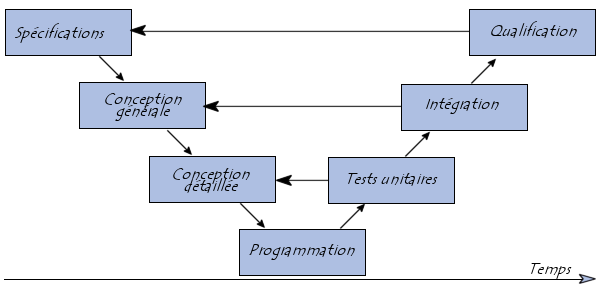
\includegraphics[width=0.66\linewidth]{img/cdv.png} 
\end{figure}

\begin{itemize}
	\item \textit{Sp\'ecifications} : \'etude de l'apprentissage symbolique, son utilisation dans la diff\'erenciation des lettres. 
	\item \textit{Conception g\'en\'erale} : \'etude d\'etaill\'e du programme \`a r\'ealiser, pr\'eparation des tests syst\`emes, des tests d'int\'egration de mise \`a jour des documents \'etablis dans l'\'etape pr\'ec\'edente.
	\item \textit{Conception d\'etaill\'e} : formation de l'architecture interne du programme, d\'efinition des composants, pr\'eparation des tests d'int\'egration et des tests unitaires, mise \`a jour des documents \'etablis dans l'\'etape pr\'ec\'edente.
	\item \textit{Programmation} : codage, documentation des composants.
	\item \textit{Tests:} R\'ealisation des tests, correction du  code si besoin.
	\item \textit{Int\'egration} : l'objectif est de d'assurer la bonne "communication" des diff\'erents modules du programme. Elle fait l'objet de tests d'int\'egration consign\'es dans un document.
	\item \textit{Qualification} : v\'erification de la conformit\'e du logiciel aux sp\'ecifications initiales.
\end{itemize}

\subsection{Gestion de la configuration}
La configuration du programme est compos\'ee des \'el\'ements suivants: le code source ex\'ecutable, les outils de d\'eveloppment, les tests utilis\'es, les documents et les donn\'ees.

Outils de travail collaboratif:
\begin{itemize}
	\item \textbf{SVN}: permet de partager le code source d'un logiciel, de disposer d'un historique de toutes les modifications, et d'int\'egrer facilement les modifications de fichier d'un d\'eveloppeur avant de les mettre \`a disposition des autres utilisateurs.
	\item \textbf{Doxygen}: permet de cr\'eer de la documentation \`a partir
du code source du programme. Pour cela, il tient compte de la grammaire du
langage dans lequel est \'ecrit le code source (ici, C++) ainsi que des
commentaires s'ils sont \'ecrits dans un format particulier.
	\item \textbf{Environnement technique}: le d\'eveloppement sera effectu\'e sous l'environnement GNU/Linux (Ubuntu).
\end{itemize}

\subsection{Gestion des modifications}
Les modifications peuvent avoir deux origines:
\begin{itemize}
	\item d\'etection d'une anomalie: il faut en trouver la source puis la corriger dans le plus bref d\'elai,
	\item demande d'\'evolution: il faut dans un premier temps r\'ealiser un \'etude de faisabilit\'e, pour ensuite modifier le programme en cons\'equence si cela s'av\`ere r\'ealisable dans les d\'elais impartis.
\end{itemize}
